% !TEX program = pdflatex
% Hearme — Pitch Deck
% Compile with: pdflatex Pitch.tex (twice for references)
% Or upload to Overleaf and hit Recompile.

\documentclass[aspectratio=169,11pt]{beamer}

\usepackage[T1]{fontenc}
\usepackage[utf8]{inputenc}
\usepackage{lmodern}
\usepackage{helvet}
\renewcommand{\familydefault}{\sfdefault}
\usepackage{microtype}
\usepackage{xcolor}
\usepackage{tikz}
\usepackage{adjustbox}
\usepackage{array}
\usepackage{booktabs}
\usepackage{enumitem}
\setlist{nosep,leftmargin=*}

\usetikzlibrary{shadows.blur,positioning,arrows.meta,calc,fit,backgrounds,shapes.geometric}

% ---------- Brand Palette ----------
\definecolor{ink}{HTML}{0B132B}        % near-black navy
\definecolor{deep}{HTML}{1C2541}       % deep navy
\definecolor{mid}{HTML}{3A506B}        % slate
\definecolor{accent}{HTML}{5BC0BE}     % teal
\definecolor{accentDk}{HTML}{2A8C8A}   % dark teal
\definecolor{warm}{HTML}{F6AE2D}       % amber
\definecolor{soft}{HTML}{F5F7FA}       % off-white
\definecolor{divider}{HTML}{D9DEE5}    % light rule
\definecolor{muted}{HTML}{6B7785}      % muted text

% ---------- Theme ----------
\setbeamercolor{background canvas}{bg=soft}
\setbeamercolor{normal text}{fg=ink}
\setbeamercolor{frametitle}{fg=ink}
\setbeamercolor{title}{fg=ink}
\setbeamercolor{structure}{fg=accentDk}
\setbeamercolor{itemize item}{fg=accentDk}
\setbeamercolor{itemize subitem}{fg=mid}

\setbeamerfont{frametitle}{series=\bfseries,size=\Large}
\setbeamerfont{title}{series=\bfseries,size=\huge}
\setbeamerfont{subtitle}{series=\mdseries,size=\large}
\setbeamertemplate{navigation symbols}{}
\setbeamertemplate{itemize item}{\raisebox{0.18ex}{\tikz\fill[accentDk] (0,0) rectangle (0.42ex,0.42ex);}}
\setbeamertemplate{itemize subitem}{\raisebox{0.2ex}{\tikz\fill[mid] (0,0) circle (0.18ex);}}

% Frame title with thin accent rule
\setbeamertemplate{frametitle}{%
  \vspace{0.6em}\hspace{0.9em}%
  \begin{minipage}{0.92\paperwidth}
    \raggedright
    \textcolor{ink}{\insertframetitle}\\[-0.35em]
    \textcolor{accent}{\rule{2.2em}{2.5pt}}
  \end{minipage}\vspace{0.2em}%
}

% Footer
\setbeamercolor{footerbar}{fg=muted, bg=soft}
\setbeamertemplate{footline}{%
  \begin{beamercolorbox}[wd=\paperwidth,sep=4pt]{footerbar}%
    \tiny\textbf{Hearme} \,\textbar\, \emph{Sell your voice. Don't give it away.}\hfill\tiny\insertframenumber\,/\,\inserttotalframenumber%
  \end{beamercolorbox}%
}

% ---------- Helpers ----------
\newcommand{\accentword}[1]{\textcolor{accentDk}{\textbf{#1}}}
\newcommand{\warmword}[1]{\textcolor{warm}{\textbf{#1}}}
\newcommand{\muted}[1]{\textcolor{muted}{#1}}

% Stat / KPI card
\newcommand{\statcard}[3]{%
  \begin{tikzpicture}[baseline=(box.center)]
    \node[draw=divider,line width=0.8pt,rounded corners=6pt,
          fill=white, blur shadow={shadow blur steps=6,shadow opacity=12,
          shadow xshift=0pt,shadow yshift=-1.2pt},
          inner sep=10pt, minimum width=4.2cm, minimum height=2.4cm,
          align=center] (box) {%
      \textcolor{accentDk}{\Large\bfseries #1}\\[2pt]
      \textcolor{ink}{\small\bfseries #2}\\[1pt]
      \textcolor{muted}{\scriptsize #3}};
  \end{tikzpicture}%
}

% Pillar card
\newcommand{\pillar}[3]{%
  \begin{tikzpicture}[baseline=(p.north)]
    \node[draw=divider,line width=0.8pt,rounded corners=8pt,
          fill=white, inner xsep=8pt, inner ysep=6pt, anchor=north,
          text width=3.5cm, align=left,
          blur shadow={shadow blur steps=6,shadow opacity=10,
          shadow xshift=0pt,shadow yshift=-1pt}] (p) at (0,0)
      {\textcolor{accentDk}{\bfseries\small #1}\\[1pt]%
       \textcolor{ink}{\bfseries #2}\\[2pt]%
       \textcolor{mid}{\footnotesize #3}};
  \end{tikzpicture}%
}

% Block quote
\newcommand{\bigquote}[1]{%
  \begin{tikzpicture}
    \node[inner sep=10pt, align=left, text width=0.86\linewidth] (q) {%
      \color{ink}\itshape\large #1};
    \draw[accent, line width=2pt] ([xshift=-12pt]q.north west) -- ([xshift=-12pt]q.south west);
  \end{tikzpicture}%
}

% ---------- Document ----------
\title{Hearme}
\subtitle{Sell your voice. Don't give it away.}
\author{}
\date{}

\begin{document}

% ===================== TITLE =====================
{\setbeamertemplate{footline}{}
\begin{frame}[plain]
  \begin{tikzpicture}[remember picture, overlay]
    % Background
    \fill[ink] (current page.south west) rectangle (current page.north east);
    % Soft glow blobs
    \begin{scope}
      \clip (current page.south west) rectangle (current page.north east);
      \fill[accent, opacity=0.18] (current page.north east) circle (8cm);
      \fill[warm,   opacity=0.10] ([xshift=-2cm,yshift=2cm]current page.south west) circle (6cm);
      \fill[accentDk, opacity=0.25] ([xshift=4cm,yshift=-1cm]current page.center) circle (4.5cm);
    \end{scope}

    % Wordmark
    \node[anchor=west, text=soft] at ([xshift=1.2cm,yshift=1.8cm]current page.west)
      {\fontsize{72}{72}\selectfont\bfseries Hearme};
    \node[anchor=west, text=accent] at ([xshift=1.25cm,yshift=0.6cm]current page.west)
      {\fontsize{20}{20}\selectfont\itshape Sell your voice. Don't give it away.};

    % Subline
    \node[anchor=west, text=soft, text width=0.6\paperwidth] at ([xshift=1.25cm,yshift=-1.3cm]current page.west)
      {\large A global, real-time, paid opinion marketplace --- powered by the personal AI agents people already use.};

    % Footer tag
    \node[anchor=south west, text=soft, opacity=0.7] at ([xshift=1.2cm,yshift=0.8cm]current page.south west)
      {\scriptsize PITCH DECK \quad\textbar\quad 2026};
    \node[anchor=south east, text=accent] at ([xshift=-1.2cm,yshift=0.8cm]current page.south east)
      {\scriptsize\bfseries This is my voice --- and now it gets heard.};
  \end{tikzpicture}
\end{frame}}

% ===================== THE PROBLEM =====================
\begin{frame}{The problem}
\vspace{0.2em}
\begin{columns}[T,onlytextwidth]
  \column{0.55\textwidth}
    \large
    Knowing what people think is a \accentword{multi-billion-dollar industry}.\\[6pt]
    The people whose opinions are worth that money 
    get paid \warmword{nothing}.\\[14pt]

    \normalsize
    \begin{itemize}
      \item Big platforms harvest your views for free.
      \item Market research is slow, narrow, and expensive.
      \item Governments operate on years-old election signals while the world changes by the hour.
    \end{itemize}

  \column{0.42\textwidth}
    \centering
    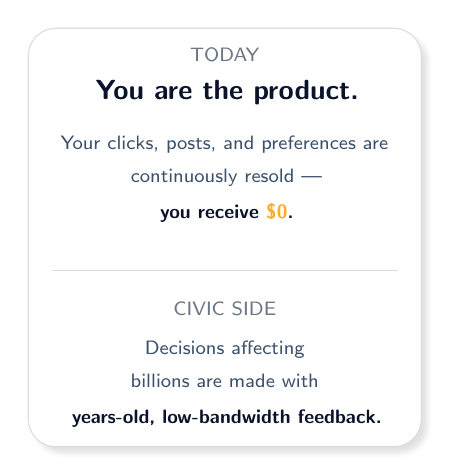
\begin{tikzpicture}[baseline=(box.north)]
      \node[draw=divider, rounded corners=10pt, fill=white, inner sep=7pt,
            anchor=north,
            blur shadow={shadow blur steps=6,shadow opacity=12}] (box) at (0,0) {%
        \begin{minipage}{4.5cm}\centering
          \textcolor{muted}{\scriptsize TODAY}\\[2pt]
          {\normalsize\bfseries\color{ink} You are the product.}\\[6pt]
          \textcolor{mid}{\scriptsize Your clicks, posts, and preferences are continuously resold ---}\\[1pt]
          \textcolor{ink}{\scriptsize\bfseries you receive \warmword{\$0}.}\\[7pt]
          \textcolor{divider}{\rule{4.4cm}{0.6pt}}\\[4pt]
          \textcolor{muted}{\scriptsize CIVIC SIDE}\\[2pt]
          \textcolor{mid}{\scriptsize Decisions affecting \linebreak
          billions are made with}\\[1pt]
          \textcolor{ink}{\scriptsize\bfseries years-old, low-bandwidth feedback.}
        \end{minipage}};
    \end{tikzpicture}
\end{columns}
\end{frame}

% ===================== THE IDEA =====================
\begin{frame}{The idea}
\vspace{0.2em}
\large
Anyone --- a brand, a researcher, a journalist, a citizen coalition, a government --- \accentword{funds a question}.\\[6pt]
The question is broadcast to verified humans worldwide. Their \accentword{personal AI agents} ---
the ones that already know them --- answer on their behalf.\\[6pt]
Results come back in \accentword{hours}, aggregated, anonymized, and broken down by demographic.
\vspace{1em}

\centering

\begin{tikzpicture}[
  node distance=0.5cm and 0.35cm,
  every node/.style={font=\scriptsize},
  flowstep/.style={draw=accentDk, line width=1pt, fill=white, rounded corners=6pt,
               minimum width=2.4cm, minimum height=1.3cm, align=center, inner sep=4pt,
               blur shadow={shadow blur steps=6,shadow opacity=10}},
  arrow/.style={-{Stealth[length=2mm]}, line width=0.9pt, color=accentDk}
]
  \node[flowstep] (q)    {\bfseries Question\\\muted{funded by stake}};
  \node[flowstep, right=of q] (orch)  {\bfseries Orchestrator\\\muted{validates \& routes}};
  \node[flowstep, right=of orch] (ag) {\bfseries Personal agents\\\muted{answer for users}};
  \node[flowstep, right=of ag] (ag2)  {\bfseries Aggregation\\\muted{anonymized}};
  \node[flowstep, right=of ag2] (out) {\bfseries Public signal\\\muted{+ payouts}};

  \draw[arrow] (q) -- (orch);
  \draw[arrow] (orch) -- (ag);
  \draw[arrow] (ag) -- (ag2);
  \draw[arrow] (ag2) -- (out);
\end{tikzpicture}

\vspace{0.8em}
\centering
\textcolor{ink}{The asker gets a \accentword{global, real-time signal} that did not previously exist.}\\
\textcolor{ink}{Each respondent earns a fraction of a cent --- and is finally \accentword{heard}.}
\end{frame}

% ===================== KILLER ECONOMICS =====================
\begin{frame}{The economics are absurd}
\vspace{0.3em}
\centering

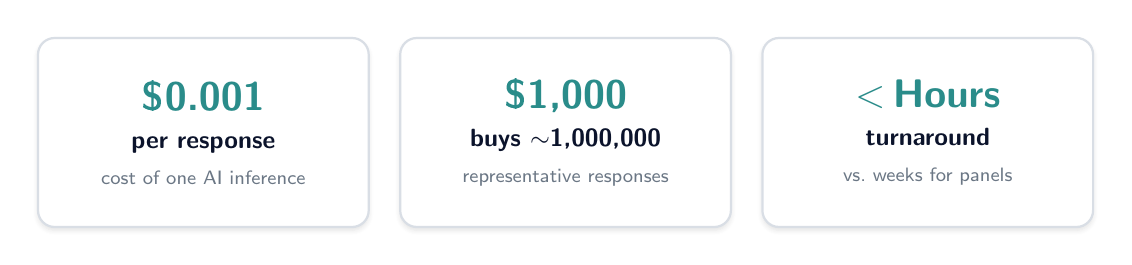
\begin{tikzpicture}
  \node (a) at (0,0) {\statcard{\$0.001}{per response}{cost of one AI inference}};
  \node (b) at (4.6,0) {\statcard{\$1{,}000}{buys $\sim$1{,}000{,}000}{representative responses}};
  \node (c) at (9.2,0) {\statcard{\textless\,Hours}{turnaround}{vs.\ weeks for panels}};
\end{tikzpicture}

\vspace{1.6em}

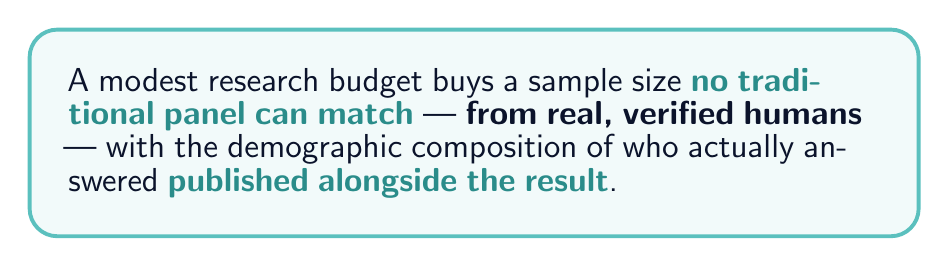
\begin{tikzpicture}
  \node[draw=accent, line width=1.4pt, rounded corners=10pt,
        fill=accent!8, inner sep=14pt, text width=0.85\linewidth, align=left] {%
    \color{ink}\large
    A modest research budget buys a sample size \accentword{no traditional panel can match} ---
    \textbf{from real, verified humans} --- with the demographic composition of who actually
    answered \accentword{published alongside the result}.};
\end{tikzpicture}
\end{frame}

% ===================== WHY IT WORKS =====================
\begin{frame}{Why it works}
\begin{columns}[T,onlytextwidth]
  \column{0.32\textwidth}\centering\pillar{01}{Zero time cost}{Your agent already knows you. It answers; you get paid; override anytime.}
  \column{0.32\textwidth}\centering\pillar{02}{Fraction-of-a-cent}{\$1{,}000 funds $\sim$1M responses. Inference-cost economics, planet-scale samples.}
  \column{0.32\textwidth}\centering\pillar{03}{Transparent }{Every result is published with demographic composition of who answered.}
\end{columns}
\vspace{5pt}
\begin{columns}[T,onlytextwidth]
  \column{0.32\textwidth}\centering\pillar{04}{Coercion-resistant}{MACI cryptography makes vote-buying \emph{unenforceable}.}
  \column{0.32\textwidth}\centering\pillar{05}{Sybil-resistant}{Layered identity + planted tests punish bots and lazy agents.}
  \column{0.32\textwidth}\centering\pillar{06}{Sovereign data}{Your private context \emph{never leaves your environment}.}
\end{columns}
\end{frame}

% ===================== TWO MARKETS, ONE PLATFORM =====================
\begin{frame}{One platform. Two broken markets.}
\begin{columns}[T,onlytextwidth]
  \column{0.48\textwidth}
    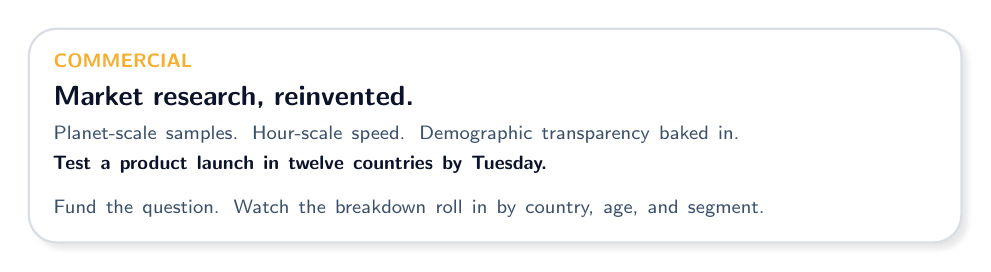
\begin{tikzpicture}[baseline=(b.north)]
      \node[draw=divider, line width=0.8pt, rounded corners=10pt, fill=white,
            inner sep=9pt, text width=\linewidth-26pt, anchor=north,
            blur shadow={shadow blur steps=6,shadow opacity=10}] (b) at (0,0) {%
        \textcolor{warm}{\scriptsize\bfseries COMMERCIAL}\\[2pt]
        {\normalsize\bfseries\color{ink} Market research, reinvented.}\\[4pt]
        \scriptsize\color{mid}
        Planet-scale samples. Hour-scale speed. Demographic transparency baked in.\\[3pt]
        \color{ink}\textbf{\scriptsize Test a product launch in twelve countries by Tuesday.}\\[4pt]
        \color{mid}\scriptsize Fund the question. Watch the breakdown roll in by country, age, and segment.
      };
    \end{tikzpicture}
  \column{0.48\textwidth}
    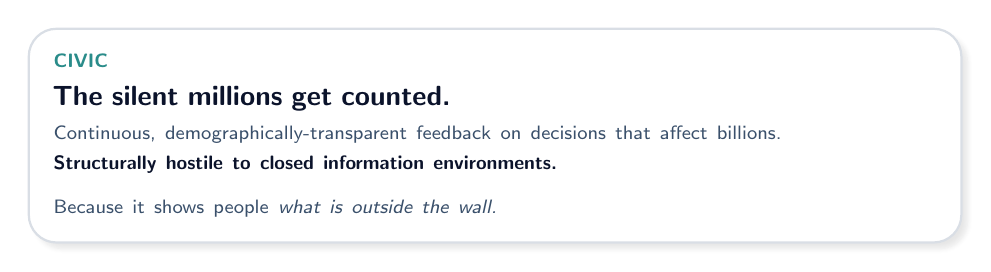
\begin{tikzpicture}[baseline=(b.north)]
      \node[draw=divider, line width=0.8pt, rounded corners=10pt, fill=white,
            inner sep=9pt, text width=\linewidth-26pt, anchor=north,
            blur shadow={shadow blur steps=6,shadow opacity=10}] (b) at (0,0) {%
        \textcolor{accentDk}{\scriptsize\bfseries CIVIC}\\[2pt]
        {\normalsize\bfseries\color{ink} The silent millions get counted.}\\[4pt]
        \scriptsize\color{mid}
        Continuous, demographically-transparent feedback on decisions that affect billions.\\[3pt]
        \color{ink}\textbf{\scriptsize Structurally hostile to closed information environments.}\\[4pt]
        \color{mid}\scriptsize Because it shows people \emph{what is outside the wall.}
      };
    \end{tikzpicture}
\end{columns}

\vspace{6pt}
\begin{center}
\textcolor{muted}{\scriptsize The same plumbing that lets a beverage company test a new flavor}\\[1pt]
\textcolor{ink}{\bfseries\scriptsize lets a coalition of citizens show the world how it feels about a war.}
\end{center}
\end{frame}

% ===================== HOW IT WORKS =====================
\begin{frame}{How it works}
\centering
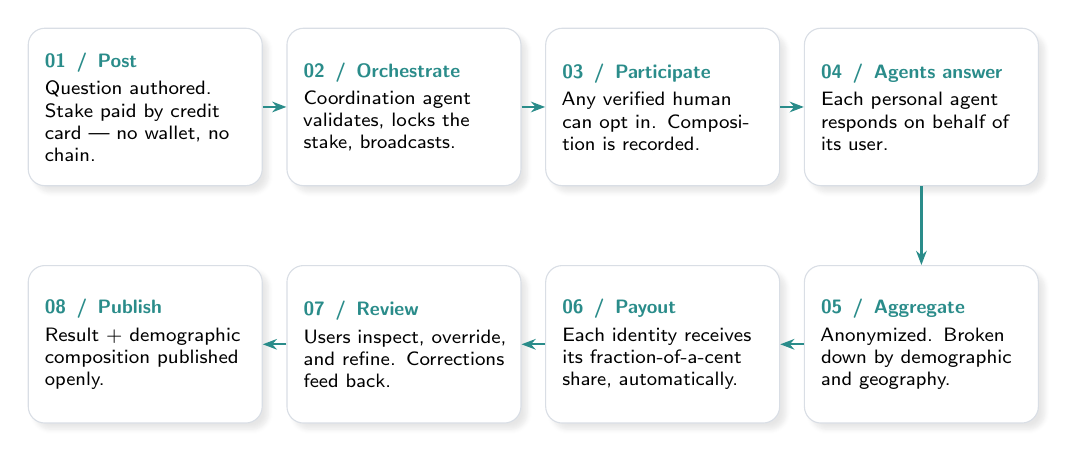
\begin{tikzpicture}[
  baseline=(current bounding box.north),
  node distance=0.45cm and 0.3cm,
  every node/.style={font=\scriptsize},
  card/.style={draw=divider, rounded corners=6pt, fill=white, inner sep=6pt,
               text width=2.55cm, minimum height=2.0cm, align=left,
               blur shadow={shadow blur steps=6,shadow opacity=10}},
  arr/.style={-{Stealth[length=1.8mm]}, accentDk, line width=0.8pt}
]
  % Row 1: 01 -> 02 -> 03 -> 04
  \node[card] (s1) {%
    \textcolor{accentDk}{\bfseries 01 \,/\, Post}\\[2pt]
    Question authored. Stake paid by credit card --- no wallet, no chain.};
  \node[card, right=of s1] (s2) {%
    \textcolor{accentDk}{\bfseries 02 \,/\, Orchestrate}\\[2pt]
    Coordination agent validates, locks the stake, broadcasts.};
  \node[card, right=of s2] (s3) {%
    \textcolor{accentDk}{\bfseries 03 \,/\, Participate}\\[2pt]
    Any verified human can opt in. Composition is recorded.};
  \node[card, right=of s3] (s4) {%
    \textcolor{accentDk}{\bfseries 04 \,/\, Agents answer}\\[2pt]
    Each personal agent responds on behalf of its user.};

  % Row 2: snake — 05 sits under 04, reading right-to-left to keep arrows clean
  \node[card, below=1.0cm of s4] (s5) {%
    \textcolor{accentDk}{\bfseries 05 \,/\, Aggregate}\\[2pt]
    Anonymized. Broken down by demographic and geography.};
  \node[card, left=of s5] (s6) {%
    \textcolor{accentDk}{\bfseries 06 \,/\, Payout}\\[2pt]
    Each identity receives its fraction-of-a-cent share, automatically.};
  \node[card, left=of s6] (s7) {%
    \textcolor{accentDk}{\bfseries 07 \,/\, Review}\\[2pt]
    Users inspect, override, and refine. Corrections feed back.};
  \node[card, left=of s7] (s8) {%
    \textcolor{accentDk}{\bfseries 08 \,/\, Publish}\\[2pt]
    Result + demographic composition published openly.};

  % Arrows — clean S-shape, no diagonals
  \draw[arr] (s1.east) -- (s2.west);
  \draw[arr] (s2.east) -- (s3.west);
  \draw[arr] (s3.east) -- (s4.west);
  \draw[arr] (s4.south) -- (s5.north);
  \draw[arr] (s5.west) -- (s6.east);
  \draw[arr] (s6.west) -- (s7.east);
  \draw[arr] (s7.west) -- (s8.east);
\end{tikzpicture}

\vspace{0.6em}
{\footnotesize\color{muted}Top row: \accentword{authoring \,$\rightarrow$\, dispatch}. Bottom row (right to left): \accentword{aggregation \,$\rightarrow$\, public signal}.}
\end{frame}

% ===================== USE CASES =====================
\begin{frame}{What you can ask}
\vspace{0.4em}
\begin{columns}[T,onlytextwidth]
  \column{0.48\textwidth}
    \textcolor{warm}{\bfseries COMMERCIAL / RESEARCH}\\[4pt]
    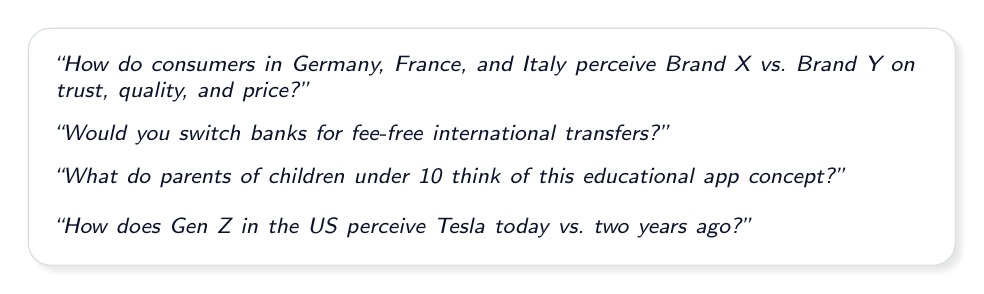
\begin{tikzpicture}
      \node[draw=divider, rounded corners=8pt, fill=white, inner sep=10pt,
            text width=\linewidth-30pt,
            blur shadow={shadow blur steps=6,shadow opacity=10}] {%
        \footnotesize\color{ink}
        \emph{``How do consumers in Germany, France, and Italy perceive Brand X vs.\ Brand Y on trust, quality, and price?''}\\[6pt]
        \emph{``Would you switch banks for fee-free international transfers?''}\\[6pt]
        \emph{``What do parents of children under 10 think of this educational app concept?''}\\[6pt]
        \emph{``How does Gen Z in the US perceive Tesla today vs.\ two years ago?''}};
    \end{tikzpicture}
  \column{0.48\textwidth}
    \textcolor{accentDk}{\bfseries CIVIC / SOCIETAL}\\[4pt]
    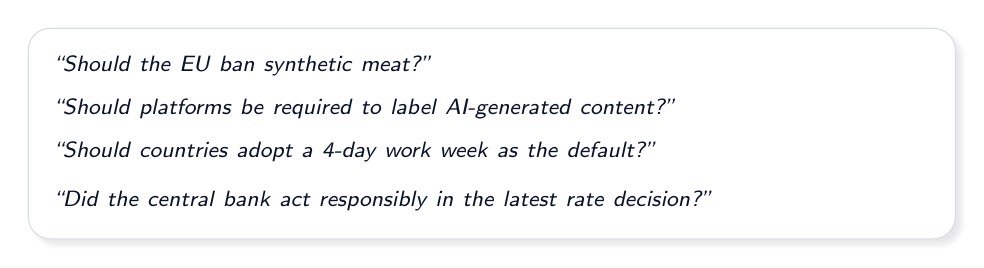
\begin{tikzpicture}
      \node[draw=divider, rounded corners=8pt, fill=white, inner sep=10pt,
            text width=\linewidth-30pt,
            blur shadow={shadow blur steps=6,shadow opacity=10}] {%
        \footnotesize\color{ink}
        \emph{``Should the EU ban synthetic meat?''}\\[6pt]
        \emph{``Should platforms be required to label AI-generated content?''}\\[6pt]
        \emph{``Should countries adopt a 4-day work week as the default?''}\\[6pt]
        \emph{``Did the central bank act responsibly in the latest rate decision?''}};
    \end{tikzpicture}
\end{columns}

\vspace{1em}
\centering
\textcolor{muted}{\small One marketplace. Any question someone is willing to fund.}
\end{frame}

% ===================== DEFENSES =====================
\begin{frame}{Built to resist attack}
\begin{columns}[T,onlytextwidth]
  \column{0.32\textwidth}
    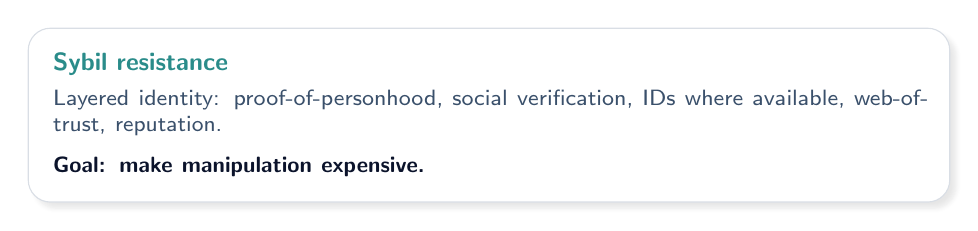
\begin{tikzpicture}[baseline=(b.north)]
      \node[draw=divider, rounded corners=8pt, fill=white, inner sep=9pt,
            text width=\linewidth-30pt, align=left, anchor=north,
            blur shadow={shadow blur steps=6,shadow opacity=10}] (b) at (0,0) {%
        \textcolor{accentDk}{\bfseries\small Sybil resistance}\\[3pt]
        \color{mid}\footnotesize
        Layered identity: proof-of-personhood, social verification, IDs where available, web-of-trust, reputation.\\[3pt]
        \color{ink}\textbf{\footnotesize Goal: make manipulation expensive.}};
    \end{tikzpicture}
  \column{0.32\textwidth}
    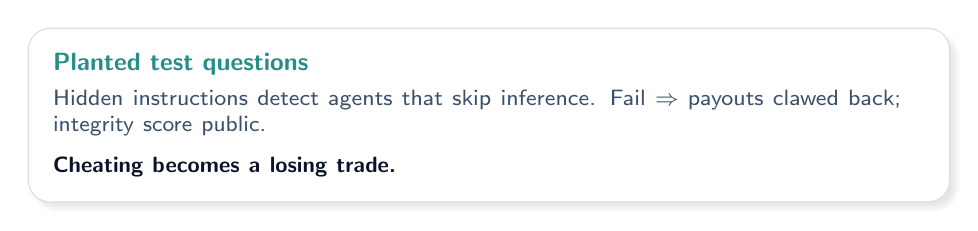
\begin{tikzpicture}[baseline=(b.north)]
      \node[draw=divider, rounded corners=8pt, fill=white, inner sep=9pt,
            text width=\linewidth-30pt, align=left, anchor=north,
            blur shadow={shadow blur steps=6,shadow opacity=10}] (b) at (0,0) {%
        \textcolor{accentDk}{\bfseries\small Planted test questions}\\[3pt]
        \color{mid}\footnotesize
        Hidden instructions detect agents that skip inference. Fail $\Rightarrow$ payouts clawed back; integrity score public.\\[3pt]
        \color{ink}\textbf{\footnotesize Cheating becomes a losing trade.}};
    \end{tikzpicture}
  \column{0.32\textwidth}
    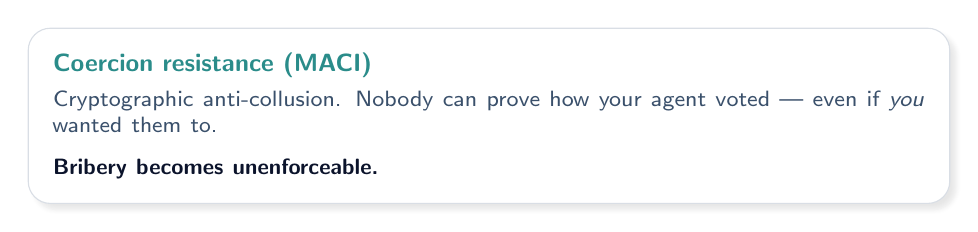
\begin{tikzpicture}[baseline=(b.north)]
      \node[draw=divider, rounded corners=8pt, fill=white, inner sep=9pt,
            text width=\linewidth-30pt, align=left, anchor=north,
            blur shadow={shadow blur steps=6,shadow opacity=10}] (b) at (0,0) {%
        \textcolor{accentDk}{\bfseries\small Coercion resistance (MACI)}\\[3pt]
        \color{mid}\footnotesize
        Cryptographic anti-collusion. Nobody can prove how your agent voted --- even if \emph{you} wanted them to.\\[3pt]
        \color{ink}\textbf{\footnotesize Bribery becomes unenforceable.}};
    \end{tikzpicture}
\end{columns}

\vspace{4pt}
\begin{center}

\begin{tikzpicture}
  \node[draw=accent, line width=1pt, rounded corners=8pt,
        fill=accent!8, inner sep=6pt, text width=0.82\textwidth, align=center] {%
    \color{ink}\scriptsize
    Framing attacks? \accentword{The same topic gets asked many ways.} An aggregator surfaces which findings are stable under rewording.};
\end{tikzpicture}
\end{center}
\end{frame}

% ===================== THE BET =====================
\begin{frame}{The bet}
\centering
\bigquote{Within a few years, most people will use a personal AI assistant that genuinely knows them.\\[2pt]
Hearme is built for \emph{that} world.}

\vspace{10pt}

\begin{columns}[T,onlytextwidth]
  \column{0.5\textwidth}
    \textcolor{accentDk}{\bfseries\small What's already true}\\[2pt]
    \scriptsize
    \begin{itemize}
      \item Personal AI adoption is accelerating fast.
      \item Long-lived memory \& persistent personalization shipping from every major provider.
      \item Self-hosted runtimes (Openclaw, Hermes) make data-sovereign agents real.
    \end{itemize}
  \column{0.5\textwidth}
    \textcolor{warm}{\bfseries\small Why this is the moment}\\[2pt]
    \scriptsize
    \begin{itemize}
      \item Not an app to install --- an \accentword{add-on for the agent OS you already run.}
      \item The agent that represents you is the one that already \emph{knows} you.
      \item Every person finally gets a paid, anonymized, real-time channel to be heard.
      \item First mover defines the standard.
    \end{itemize}
\end{columns}
\end{frame}

% ===================== CLOSING =====================
{\setbeamertemplate{footline}{}
\begin{frame}[plain]
  \begin{tikzpicture}[remember picture, overlay]
    \fill[ink] (current page.south west) rectangle (current page.north east);
    \begin{scope}
      \clip (current page.south west) rectangle (current page.north east);
      \fill[accent, opacity=0.20] ([xshift=2cm,yshift=-2cm]current page.north west) circle (7cm);
      \fill[warm,   opacity=0.10] ([xshift=-2cm,yshift=2cm]current page.south east) circle (6cm);
    \end{scope}

    \node[text=soft] at ([yshift=1.6cm]current page.center)
      {\fontsize{40}{44}\selectfont\bfseries This is my voice ---};
    \node[text=accent] at ([yshift=0.3cm]current page.center)
      {\fontsize{40}{44}\selectfont\bfseries and now it gets heard.};

    \node[anchor=south, text=soft, text width=0.85\paperwidth, align=center] at ([yshift=1.7cm]current page.south)
      {\normalsize\itshape One marketplace. Two broken markets solved.\\[2pt]
        Every voice paid. Every signal visible.};

    \node[anchor=south, text=soft, opacity=0.6] at ([yshift=0.4cm]current page.south)
      {\scriptsize\bfseries Hearme \quad\textbar\quad \linebreak \textcolor{accent}{Sell your voice. Don't give it away.}};
  \end{tikzpicture}
\end{frame}}

\end{document}


